\section{Estado del Arte}

\subsection{IA Generativa y LLMs en Operaciones Espaciales}

Resulta revelador observar cómo los modelos de lenguaje grandes han pasado en pocos años de herramientas de generación de texto a candidatos serios para toma de decisiones autónomas en entornos de alta complejidad. En el dominio espacial, particularmente, esta transición genera tanto entusiasmo como cautela justificada.

Trabajos recientes han explorado el uso de LLMs puros como operadores de naves espaciales en simuladores de alta fidelidad. Un ejemplo notable consiste en agentes basados exclusivamente en LLMs que controlan maniobras en el entorno Kerbal Space Program Differential Games, logrando desempeños competitivos en operaciones no cooperativas mediante prompting estructurado y bucles de retroalimentación \cite{Carrasco2025_LLMSpace}. Estos enfoques destacan por su flexibilidad y capacidad para razonar en lenguaje natural sobre estados de telemetría.

No obstante, cabe matizar que las fortalezas de los LLMs --generalización zero-shot y razonamiento contextual-- vienen acompañadas de limitaciones críticas en predictibilidad y consumo de recursos. Implementaciones prácticas de agentes ReAct con técnicas de Retrieval-Augmented Generation (RAG) han mostrado mayor robustez en operaciones ground/space, permitiendo a los agentes consultar documentación procedural y generar secuencias de comandos justificadas \cite{Li2025_AIAgents}. 

Aunque prometedores, estos sistemas tienden a exhibir alucinaciones en escenarios edge-case, lo que plantea interrogantes serios sobre su despliegue directo en misiones críticas sin capas de verificación formal.

\subsection{Agentes Autónomos y MARL para OSAM}

Uno de los desafíos persistentes al analizar operaciones de servicio en órbita radica en la coordinación efectiva bajo dinámica orbital incierta y comunicaciones limitadas. Aquí, los enfoques basados en reinforcement learning multi-agente (MARL) han ganado terreno significativo.

Entornos de simulación como OrbitZoo han facilitado el desarrollo y benchmarking de estrategias MARL en escenarios realistas que incluyen evitación de colisiones, maniobras cooperativas y transferencias orbitales con perturbaciones completas \cite{Oliveira2025_OrbitZoo}. Estos benchmarks revelan que las políticas descentralizadas pueden lograr comportamientos emergentes útiles, aunque a costa de convergencia lenta y sensibilidad a la inicialización.

En paralelo, frameworks específicos de RL para On-Orbit Servicing demuestran que un servicer autónomo puede aprender a detectar riesgos de colisión, rendezvous y ejecutar maniobras de avoidance óptimas integrando estimaciones de riesgo y datos de debris \cite{Patnala2024_OOS_RL}. 

\begin{table*}[t]
\centering
\caption{Comparativa de enfoques MARL en operaciones orbitales}
\label{tab:marl_comparison}
\begin{tabular}{lcccc}
\hline
Enfoque & Escenario Principal & Robustez Perturbaciones & Escalabilidad Agentes & Consumo Computacional \\
\hline
RL Single-Agent & CAM simple & Media & Baja & Bajo \\
MARL Independiente & Coordinación GEO & Alta en sim. & Media & Alto \\
MARL Federated & Transferencias cooperativas & Alta & Alta & Medio \\
\textbf{Híbrido Generativo+MARL (tendencia)} & OSAM completo & Muy alta & Alta & Medio-Alto \\
\hline
\end{tabular}
\end{table*}

La Tabla 2 sintetiza estas tendencias y subraya brechas que el marco propuesto busca abordar.

\subsection{Arquitecturas de Referencia para Serviciado Autónomo}

Lejos de ser un asunto resuelto, la integración de capacidades generativas con control clásico en arquitecturas de referencia para OSAM sigue representando un territorio en exploración activa. Muchos trabajos se centran en componentes aislados --ya sea planificación o ejecución-- dejando sin resolver la cuestión de la orquestación completa a nivel de sistema.

Particularmente llamativo es el hecho de que, mientras los entornos MARL proporcionan realismo dinámico, rara vez incorporan la flexibilidad semántica y de razonamiento de alto nivel que ofrecen los LLMs. Esta desconexión constituye una brecha clave identificada en la literatura reciente.

\begin{figure}[t]
\centering
% 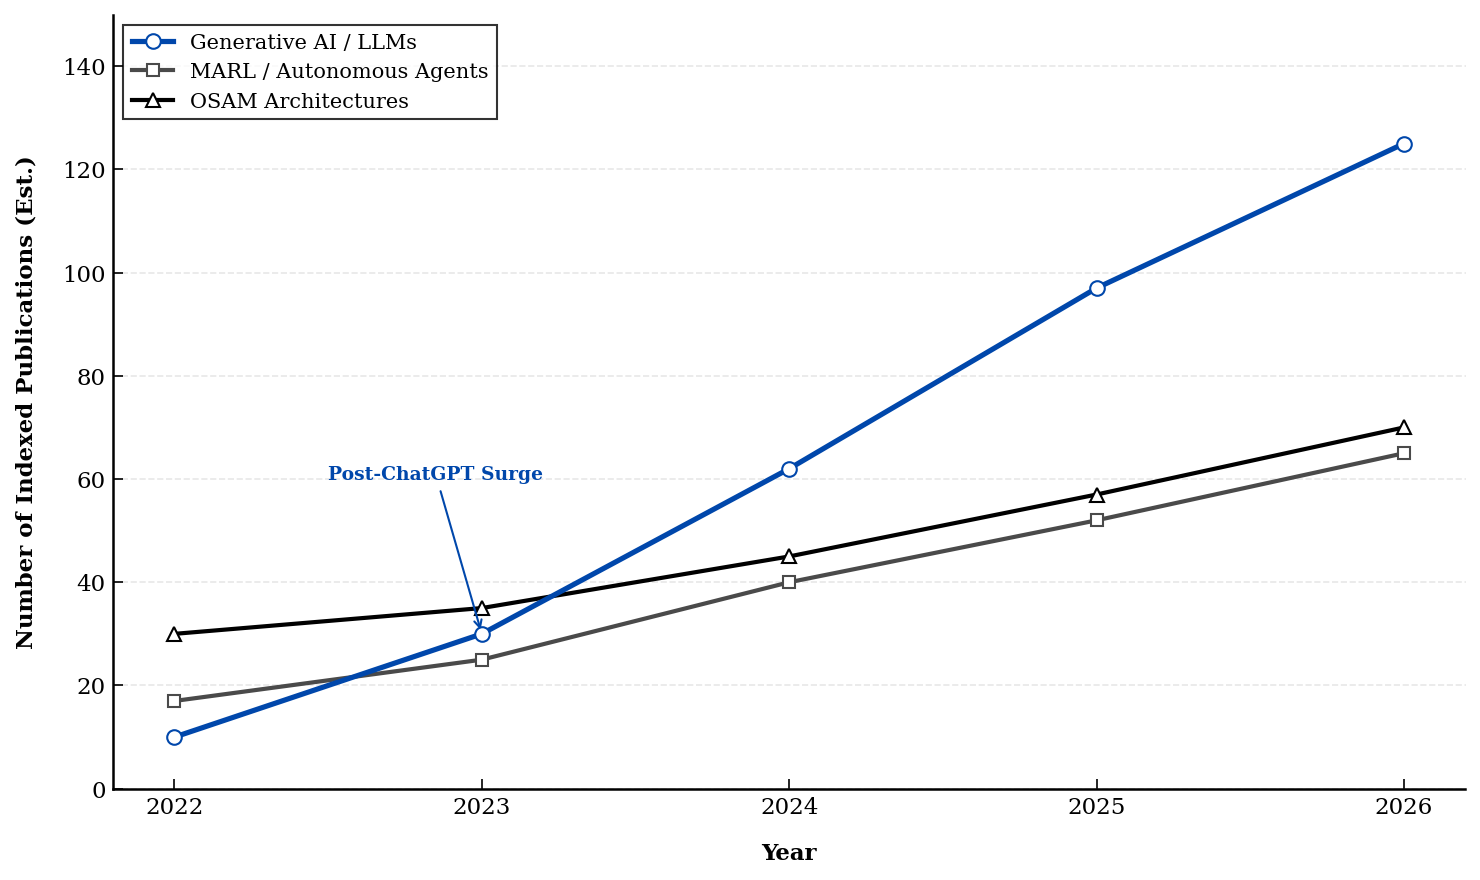
\includegraphics[width=0.95\linewidth]{fig2.png}
\scalebox{1}{\definecolor{cobaltblue}{HTML}{0047AB}
\definecolor{techgray}{HTML}{4A4A4A}
\begin{tikzpicture}
\begin{axis}[
    width=\linewidth,
    height=8cm,
    grid=major,
    grid style={dashed, gray!30},
    xlabel={\textbf{Year}},
    ylabel={\textbf{Number of Indexed Publications (Est.)}},
    xmin=2022, xmax=2026,
    ymin=0, ymax=150,
    xtick={2022, 2023, 2024, 2025, 2026},
    legend pos=north west,
    legend style={draw=black, fill=white, font=\footnotesize, cells={anchor=west}},
    axis x line=bottom,
    axis y line=left,
    clip=false % Importante para permitir anotaciones fuera del eje
]

% Serie Gen AI / LLMs
\addplot[cobaltblue, thick, mark=*, mark options={fill=white}] coordinates {(2022,10)(2023,30)(2024,62)(2025,97)(2026,125)};
\addlegendentry{Generative AI / LLMs}

% Serie MARL / Agents
\addplot[techgray, thick, mark=square*, mark options={fill=white}] coordinates {(2022,17)(2023,25)(2024,40)(2025,52)(2026,65)};
\addlegendentry{MARL / Autonomous Agents}

% Serie OSAM Archs
\addplot[black, thick, mark=triangle*, mark options={fill=white}] coordinates {(2022,30)(2023,35)(2024,45)(2025,57)(2026,70)};
\addlegendentry{OSAM Architectures}

% Anotación Post-ChatGPT Surge
\draw[->, cobaltblue, thick] (axis cs:2022.6, 55) -- (axis cs:2023, 32);
\node[cobaltblue, font=\scriptsize\bfseries, anchor=south] at (axis cs:2022.7, 55) {Post-ChatGPT Surge};

\end{axis}
\end{tikzpicture}

}
\caption{Evolución temporal de publicaciones en IA generativa, MARL y arquitecturas autónomas para operaciones espaciales (2022-2026).}
\label{fig:publications_evolution}
\end{figure}

En conjunto, el estado del arte muestra avances prometedores pero fragmentados. La mayoría de las propuestas exhiben fortalezas en dominios específicos, sin embargo carecen de un marco unificado que combine generación de planes, aprendizaje multi-agente y garantías de seguridad verificables para operaciones OSAM reales. Esta observación motiva directamente la arquitectura híbrida que desarrollamos en las secciones siguientes.